\documentclass[./skripsi.tex]{subfiles}
\begin{document}
\chapter{Tinjauan Pustaka dan Landasan Teori}
\section{Tinjauan Pustaka}
\subsection{Penelitian 1 : Penerapan metode statistik dan neural network pada Intrusion Detection System}
\par Pada Penelitian Zhang, tentang pendeteksian menggunakan metode statistik dan  \textit{Neural Network} pada Intrusion Detection System untuk pendeteksian intrusi pada sisi serangan protokol UDP. Pengujian dilakukan dengan menggunakan beberapa jenis neural network antara lain Perceptron, Backpropagation, PBH, Fuzzy ARTMAP, dan Radial-based Function.
\par Akurasi tertinggi dicapai oleh Backpropagation, dan PBH (Perceptron Backpropagation Hybrid), dimana MSR errornya berkurang seiring dengan jumlah data yang dimasukkan yang berkisar di 5\% sampai 10\% dari intensitas data background.\cite{zhang2001hide}
\subsection{Penelitian 2 : Penerapan Kecerdasan Buatan pada Intrusion Detection System}
\par Pada penelitian I Nyoman Trisna Wirawan, dan Ivan Eksistyanto tentang penerapan kecerdasan buatan pada IDS.Penelitian ini menggunakan salah satu metode Machine Learning yakni Naive Bayes memperoleh akurasi sebesar 89\% dengan running time. 
\par Penelitian ini menerapkan \textit{Naive Bayes Classifier} dengan memilah atribut berdasarkan korelasi, dan menggunakan mean/standar deviasi untuk atribut kontinyu pada 3-interval dan 5-interval. Metode ini memperoleh akurasi sebesar 89\% dengan running time rata-rata 31 detik. \cite{wirawan2015penerapan}
\subsection{Penelitian 3 : Penerapan Metode SVM pada Intrusion Detection System secara Realtime}
\par Pada Penelitian Jacobus, tentang penerapan metode Support Vector Machine pada Intrusion Detection System secara Realtime menerapkan 3 kelas untuk proses pendeteksian jenis intrusi yakni normal, probe, dan DoS.
\par Untuk beberapa tipe intrusi dapat terdeteksi dengan akurasi diatas 90\%, dengan memanfaatkan kluster pada beberapa jenis faktor parameter dari header packet yang diperoleh dari hasil data mining. \cite{jacobus2014penerapan}

\subsection{Penelitian ini : Penerapan Metode Hybrid CNN+RNN pada Intrusion Detection System secara RealTime}
\par Pada penelitian ini akan diterapkan CNN dan RNN yang menggabungkan sistem pendeteksian berdasarkan pola dengan CNN, dan anomali dengan RNN. Proses data mining dilakukan oleh SnortIDS yang berperan sebagai daemon yang akan berjalan dibelakang saat startup. Metode ini menggabungkan time series prediction dan memanfaatkan fungsi CNN yang dapat mendeteksi pola berdasarkan jarak relatif dikarenakan perbedaan pola pada raw data saat dikirimkan dalam bentuk packet jaringan.
\par Penelitian ini dibuat untuk memaksimalkan sistem filtrasi packet dengan CNN dan performa pendeteksian dinamis menggunakan RNN yakni jenis LSTM. Penelitian ini diharapkan mampu mengintegrasikan sistem pendeteksi intrusi dengan metode \textit{Deep Learning Hybrid CNN+RNN}
\section{Landasan Teori}
\subsection{Data pada jaringan}
Data pada jaringan berbentuk Frame Ethernet dengan ukuran \textit{Maximum Transmission Unit} (MTU) tiap frame sebesar 1500 bytes. Untuk transmisi data lebih besar dari 1500 bytes akan dilakukan pemecahan per frame.
\subsection{Deep Learning}
\par 
Banyak masalah dalam penerapan kecerdasan buatan adalah bahwa banyak faktor variasi yang dapat memengaruhi setiap bagian dari data yang dapat kita amati. Contohnya, masing-masing piksel dalam gambar sebuah mobil merah mungkin menyerupai dengan mobil hitam saat di malam hari. Bentuk bayangan mobil tergantung pada sudut pandang. Sebagian besar penerapan kecerdasan buatan mengharuskan kita untuk memisahkan faktor-faktor variasi dan membuang faktor-faktor yang dapat diabaikan.
\par Sangat sulit untuk mengekstrak fitur abstrak seperti itu dari data mentah. Banyak dari faktor variasi ini, seperti aksen pembicara, dapat diidentifikasi hanya dengan menggunakan pemahaman data biasa secara manual dengan bantuan manusia. Ketika untuk mendapatkan representasi hampir sama sulitnya daripada memecahkan masalah yang seharusnya, maka dapat disimpulkan bahwa metode biasa tidak akan dapat membantu.
\par Deep Learning memecahkan masalah ini saat proses pembelajaran representasi dengan memperkenalkan representasi yang diekspresikan dalam bentuk representasi lain yang lebih sederhana. Deep Learning memungkinkan komputer untuk membangun konsep kompleks dari konsep yang sederhana.
\par Deep learning merupakan salah satu penerapan dari Machine Learning yang digunakan untuk memahami data yang memiliki makna. Contohnya seperti gambar, suara, maupun bentuk data lain yang dapat diinterpretasikan tidak secara matematis. Deep Learning memanfaatkan konsep matematis pada Machine Learning untuk mempelajari data yang lebih kompleks. nyata.\cite{goodfellow2016deep}
\subsection{Jaringan Syaraf Tiruan}
\par Jaringan saraf tiruan dipandang di sini sebagai model komputasi paralel, dengan berbagai tingkat kompleksitas, terdiri dari unit pemrosesan adaptif yang saling berhubungan. Jaringan ini adalah implementasi paralel halus dari sistem statis atau dinamis nonlinear. Fitur yang sangat penting dari jaringan ini adalah sifat adaptifnya, di mana "belajar dengan contoh" menggantikan "pemrograman" tradisional dalam menyelesaikan masalah. Fitur ini membuat model komputasi seperti itu sangat menarik dalam domain aplikasi di mana orang memiliki sedikit atau tidak lengkap pemahaman masalah yang harus dipecahkan tetapi di mana data pelatihan tersedia. Fitur utama lainnya adalah paralelisme intrinsik yang memungkinkan perhitungan solusi yang cepat ketika jaringan ini diimplementasikan pada komputer digital paralel atau, pada akhirnya, ketika diimplementasikan dalam perangkat keras khusus.
\par Jaringan syaraf tiruan adalah model komputasi yang layak untuk berbagai masalah, termasuk klasifikasi pola, sintesis dan pengenalan ucapan, antarmuka adaptif antara manusia dan sistem fisik yang kompleks, perkiraan fungsi, kompresi data gambar, memori asosiatif, pengelompokan, peramalan dan prediksi, optimisasi kombinatorial , pemodelan sistem nonlinear, dan kontrol. Jaringan-jaringan ini neural dalam arti bahwa mereka mungkin telah terinspirasi oleh ilmu saraf, tetapi bukan karena mereka adalah model yang setia dari fenomena saraf atau kognitif biologis. Faktanya, sebagian besar model jaringan yang tercakup dalam buku ini lebih erat kaitannya dengan matematika tradisional dan / atau model statistik seperti algoritma optimisasi, pengklasifikasi pola nonparametrik, algoritma pengelompokan, filter linear dan nonlinier, dan model regresi statistik daripada model neurobiologis. \cite{hassoun1995fundamentals}
\subsection{CNN}

\par CNN merupakan salah satu metode artificial neural network yang biasa diterapkan untuk data dalam bentuk gambar.
Pada CNN data gambar melalui proses ekstraksi fitur dimana, setiap piksel dari gambar akan diubah dalam bentuk data matriks angka.
Pada proses ekstraksi fitur gambar akan melalui dua layer yakni Convolutional Layer dan Pooling Layer.

\par Convolutional layer terdiri dari neuron yang tersusun sehingga membentuk sebuah filter dengan ukuran lebar, tinggi, dan tebal piksel.
Misalnya ukuran Convolutional Layer 5x5x3, atau panjang 5 piksel, tinggi 5 piksel dan tebal 3 yang merupakan channel dari gambar dersebut dalam bentuk representasi RGB.

\par Filter ini kemudian akan digeser ke seluruh bagian dari gambar yang kemudian akan di lakukan operasi perkalian antara input dan nilai dari filter sehingga menghasilkan
output yang disebut feature map.

\par Parameter pada convolutional layer, salah satunya adalah Stride. Stride adalah parameter yang menentukan jumlah pergeseran filter.
Jika nilai stride 1, maka filter akan bergeser sebanyak 1 piksel.
[Tambah penjelassan stride pada CNN]

\par Semakin kecil stride maka akan semakin detil informasi yang diperoleh dari input.
Padding merupakan parameter yang menentukan jumlah piksel (bernilai 0) yang akan ditambahkan di setiap sisi dari input. Hal ini digunakan dengan tujuan untuk memanipulasi output dari feature map.
\par Pooling Layer merupakan layer CNN yang berada setelah Convolutional Layer. Pooling layer merupakan sebuah filter yang bergeser juga pada seluruh area feature map.
\par Pada setiap pergeseran filter, nilai maksimum akan diambil sebesar ukuran dari filter. Contoh apabila menggunakan max pooling 2x2 dengan stride 2
maka setiap pergeseran filter, nilai maksimum pada area 2x2 akan dipilih, sedangkan Average Pooling memilih nilai rata-rata.

\subsection{LSTM}
\par LSTM (Long short-term memory) memiliki kemampuan untuk melupakan informasi yang tidak relevan pada jaringan RNN (recurrent neural network). LSTM merupakan RNN yang terdiri dari 4 bagian yakni, cell state, input gate, output gate, dan forget gate. Cell state merupakan bobot dari hidden layer. Input gate merupakan jalur nilai input datang. Forget gate merupakan jalur yang berfungsi untuk meniadakan atau melupakan informasi yang datang. Output gate merupakan jalur keluaran berdasarkan cell state setelah forget gate dilewati.

{\centering
\makebox {
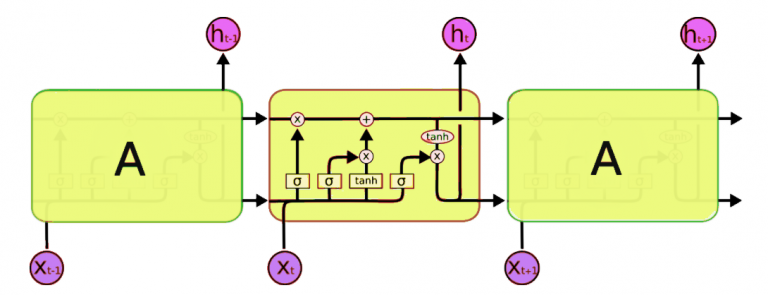
\includegraphics[width=\textwidth]{skripsi/public/assets/img/LSTM1.png}
}\captionof{figure}{Layer LSTM}}

\par Suatu sel \textit{Long Short Term Memory} mengandung empat komponen yakni komponen gate \textit{input gate}, \texit{output gate}, dan \textit{forget gate}, dan juga komponen \textit{cell state}. Keempat komponen ini masing-masing memiliki perannya sendiri.

\subsubsection{Forget Gate}
\par \textit{Forget Gate} bertanggung jawab untuk menghapus informasi dari status sel. Informasi yang tidak lagi diperlukan untuk LSTM atau informasi yang kurang penting dihapus melalui gerbang ini. Hal Ini diperlukan untuk mengoptimalkan kinerja jaringan LSTM.

\begin{center}
\makebox {
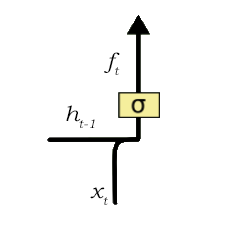
\includegraphics[width=0.5\textwidth]{skripsi/public/assets/img/ForgetGate1.png}
}\captionof{figure}{Forget Gate}
\end{center}

\par Gerbang ini menerima dua input $h_{t-1}$ dan $x_t$.
\par $h_{t-1}$ adalah keadaan tersembunyi dari sel sebelumnya atau output dari sel sebelumnya dan $x_t$ adalah input pada langkah waktu tertentu. Input yang diberikan dikalikan dengan matriks bobot dan kemudian bias ditambahkan. Setelah itu, fungsi sigmoid diterapkan ke nilai ini. Fungsi sigmoid menghasilkan vektor, dengan nilai mulai dari 0 hingga 1, sesuai dengan setiap angka dalam keadaan sel. Pada dasarnya, fungsi sigmoid bertanggung jawab untuk memutuskan nilai mana yang harus disimpan dan mana yang harus dibuang. Jika ‘0’ adalah output untuk nilai tertentu dalam keadaan sel, itu berarti \textit{forget gate} ingin keadaan sel melupakan informasi itu sepenuhnya. Demikian pula, '1' berarti bahwa \textit{forget gate} ingin mengingat seluruh informasi itu. Output vektor ini dari fungsi sigmoid dikalikan ke keadaan sel.

\subsubsection{Input Gate}
\par \textit{Input Gate} bertanggung jawab untuk penambahan informasi ke status sel. Penambahan informasi ini pada dasarnya adalah proses tiga langkah seperti yang terlihat dari diagram di atas.
\begin{center}
\makebox {
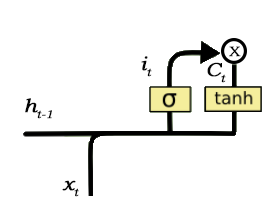
\includegraphics[width=0.5\textwidth]{skripsi/public/assets/img/InputGate1.png}
}\captionof{figure}{Input Gate}
\end{center}

\begin{enumerate}
    \item Mengatur nilai apa yang perlu ditambahkan ke keadaan sel dengan melibatkan fungsi sigmoid. Ini pada dasarnya sangat mirip dengan gerbang lupa dan bertindak sebagai filter untuk semua informasi dari $h_{t-1}$ dan $x_{t}$.
    \item Membuat vektor yang berisi semua nilai yang mungkin yang dapat ditambahkan (seperti yang dirasakan dari $h_{t-1}$ dan $x_t$. Hal ini dilakukan dengan menggunakan fungsi tanh, yang menampilkan nilai dari -1 hingga +1.
    \item Mengalikan nilai filter pengaturan (gerbang sigmoid) ke vektor yang dibuat (fungsi tanh) dan kemudian menambahkan informasi berguna ini ke \textit{cell state} melalui operasi penambahan.
    \item Setelah proses tiga langkah ini selesai, layer memastikan bahwa hanya informasi yang ditambahkan ke keadaan sel yang relevan.
\end{enumerate}
\subsubsection{Output Gate}
\begin{center}
\makebox {
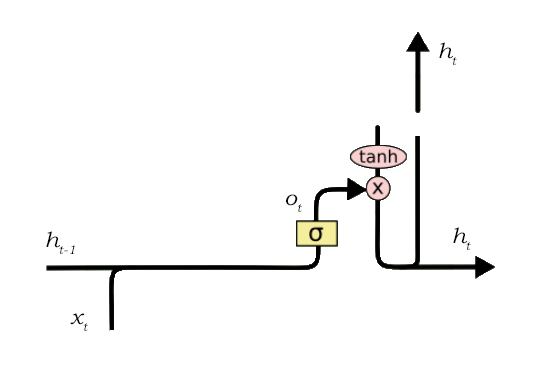
\includegraphics[width=0.5\textwidth]{skripsi/public/assets/img/OutputGate1.png}
}\captionof{figure}{Output Gate}
\end{center}
\par Fungsi gerbang keluaran dapat dipecah lagi menjadi tiga langkah:
\begin{enumerate}
    \item Membuat vektor setelah menerapkan fungsi tanh ke status sel, sehingga menskalakan nilai ke rentang -1 hingga +1.
    \item Membuat filter menggunakan nilai-nilai $h_{t-1}$ dan $x_t$, sehingga dapat mengatur nilai-nilai yang perlu dikeluarkan dari vektor yang dibuat di atas. Filter ini lagi menggunakan fungsi sigmoid.
    \item  Mengalikan nilai filter pengaturan ini ke vektor yang dibuat pada langkah 1, dan mengirimkannya sebagai output dan juga ke keadaan tersembunyi sel berikutnya.
\end{enumerate}
Filter dalam contoh di atas akan memastikan bahwa itu mengurangi semua nilai lain kecuali ‘Bob’. Jadi filter perlu dibangun pada input dan nilai-nilai kondisi tersembunyi dan diterapkan pada vektor status sel.
\cite{gers1999learning}
\subsection{IDS}
\par Sistem deteksi intrusi (IDS) adalah perangkat atau aplikasi perangkat lunak yang memantau jaringan atau sistem untuk aktivitas jahat atau pelanggaran kebijakan. Setiap aktivitas atau pelanggaran berbahaya biasanya dilaporkan kepada administrator atau dikumpulkan secara terpusat menggunakan sistem informasi keamanan dan manajemen kejadian (SIEM). Sistem SIEM menggabungkan output dari berbagai sumber, dan menggunakan teknik penyaringan alarm untuk membedakan aktivitas berbahaya dari alarm palsu. \cite{martellini2017cyber}
\par Tipe IDS berkisar dalam ruang lingkup dari satu komputer ke jaringan besar. \cite{axelsson2000intrusion} Klasifikasi yang paling umum adalah sistem deteksi intrusi jaringan (NIDS) dan sistem deteksi intrusi berbasis host (HIDS). Sistem yang memantau file sistem operasi penting adalah contoh dari HIDS, sedangkan sistem yang menganalisis lalu lintas jaringan yang masuk adalah contoh dari NIDS. Dimungkinkan juga untuk mengklasifikasikan IDS dengan pendekatan deteksi: varian yang paling terkenal adalah deteksi berbasis tanda tangan (mengenali pola-pola buruk, seperti malware); dan deteksi berbasis anomali (mendeteksi penyimpangan dari model lalu lintas "baik", yang sering bergantung pada pembelajaran mesin), yang lain adalah deteksi berbasis reputasi (mengenali potensi ancaman sesuai dengan skor reputasi). Beberapa produk IDS memiliki kemampuan untuk menanggapi intrusi yang terdeteksi. Sistem dengan kemampuan respons biasanya disebut sebagai sistem pencegahan intrusi. \cite{newman2009computer} Sistem deteksi intrusi juga dapat melayani tujuan tertentu dengan menambahkannya dengan alat khusus, seperti menggunakan honeypot untuk menarik dan mengkarakterisasi lalu lintas berbahaya.
\cite{liao2013intrusion}
\subsection{Snort IDS}
Snort adalah sistem deteksi intrusi jaringan open source (IDS) dan sistem pencegahan intrusi (IPS) \cite{carr2007snort} yang dibuat pada tahun 1998 oleh Martin Roesch, pendiri dan mantan CTO Sourcefire. \cite{greenemeier2006sourcefire} Snort sekarang dikembangkan oleh Cisco, yang membeli Sourcefire pada 2013.
\subsubsection{Cara kerja}
Sistem deteksi / pencegahan intrusi (IDS / IPS) berbasis jaringan sumber terbuka milik Snort memiliki kemampuan untuk melakukan analisis lalu lintas waktu-nyata dan pendataan paket pada jaringan Internet Protocol (IP). Snort melakukan analisis protokol, pencarian konten, dan pencocokan.

Program ini juga dapat digunakan untuk mendeteksi probe atau serangan, termasuk, tetapi tidak terbatas pada, upaya sidik jari sistem operasi, serangan URL semantik, buffer overflows, probe blok pesan server, dan pemindaian port siluman. \cite{stanger2011cheat}

Snort dapat dikonfigurasi dalam tiga mode utama: sniffer, packet logger, dan deteksi intrusi jaringan. Dalam mode sniffer, program akan membaca paket jaringan dan menampilkannya di konsol. Dalam mode packet logger, program akan mencatat paket-paket ke disk. Dalam mode deteksi intrusi, program akan memonitor lalu lintas jaringan dan menganalisanya terhadap aturan yang ditetapkan oleh pengguna. Program kemudian akan melakukan tindakan spesifik berdasarkan apa yang telah diidentifikasi.
\subsection{Flask}
\par Flask adalah framework web yang dibuat dengan Python. framework ini termasuk dalam kategori \textit{microservice} karena tidak memerlukan \textit{tools} atau \texit{library} tertentu.
\par Flask tidak memiliki lapisan abstraksi untuk basis data, validasi formulir, dan juga tidak memiliki \textit{third-party library} yang menyediakan fungsi umum. 
\par Flask mendukung ekstensi yang dapat menambahkan fitur aplikasi sehingga dapat diimplementasikan dalam Flask itu sendiri. Ekstensi yang ada seperti \textit{Object Relational Mappers}, \textit{Form Validation}, dan \textit{upload handling}. Ekstensi flask lebih sering diperbaharui dari \textit{core} flask sendiri.
\end{document}